\documentclass[a4paper]{article}
\usepackage{student}
\usepackage{graphicx}
\usepackage{mathrsfs}
\usepackage{cancel}

% Metadata
\date{\today}

%-------------------------------%
% Other details
% TODO: Fill these
%-------------------------------%
\title{Taller 3}
\setmembername{Cristian Perez} 

%-------------------------------%
% Add / Delete commands and packages
% TODO: Add / Delete here as you need
%-------------------------------%
\usepackage{amsmath,amssymb,bm}
\usepackage[spanish]{babel}

% Custom your usual commands here. Renew these.
\newcommand{\KL}{\mathrm{KL}}
\newcommand{\R}{\mathbb{R}}
\newcommand{\E}{\mathbb{E}}
\newcommand{\T}{\top}
\newcommand{\expdist}[2]{%
        \normalfont{\textsc{Exp}}(#1, #2)%
    }
\newcommand{\expparam}{\bm \lambda}
\newcommand{\Expparam}{\bm \Lambda}
\newcommand{\natparam}{\bm \eta}
\newcommand{\Natparam}{\bm H}
\newcommand{\sufstat}{\bm u}

% Main document
\begin{document}
    % Add header
    \header{}

    % Use `answer` environment to add solutions
    % \begin{answer}[Question 1.1] for example starts an environment formatted
    % for Question 1.1
    15. Demostrar directamente que la transformación
$$
\begin{gathered}
Q=\arctan \frac{\alpha q}{p}, \\
P=\frac{\alpha q^2}{2}\left(1+\frac{p^2}{\alpha^2 q^2}\right)
\end{gathered}
$$
es canónica, donde $\alpha$ es una constante.
    \begin{answer}[Problema 1]
       Sean en  $(p,q)$ la coordenadas generalizadas de un sistema en el espacion de fase, y sea $H(p,q)$ la funcion de Hamilton, entonces las ecuaciones de Hamilton son:
        
        \begin{align*}
            \dot p &= -\frac{\partial H}{\partial q}, \quad \dot q = \frac{\partial H}{\partial p} \quad \text{y} \quad  \frac{\partial H}{\partial t} =0  \quad (15.1)
        \end{align*}

        Dado que la transformacion puntual de coordenadas generalizadas $(p,q)$ a coordenadas generalizadas $(P,Q)$ dada por:
        \begin{equation*}
            \begin{align*}  
                Q&=\arctan \frac{\alpha q}{p}, \\
                P&=\frac{\alpha q^2}{2}\left(1+\frac{p^2}{\alpha^2 q^2}\right) = \frac{1}{2}\left(\alpha q^2 + \frac{p^2}{\alpha} \right)
            \end{align*} \quad (15.2)
        \end{equation*}
      
        es canónica, entonces deben satisfacer las ecuaciones de Hamilton (15.1) con $K(P,Q) = K$ constante, es decir:
        \begin{align*}
            \dot P &= -\frac{\partial K}{\partial Q} \quad \text{y} \quad \dot Q = \frac{\partial K}{\partial P}  \quad \text{y} \quad \frac{\partial K}{\partial t} =0  \quad (15.3)
        \end{align*}

        Para mostrar esto ultimo, usando la regla de la cadena en la ecuaciones (15.2) y reemplazando (15.1)
        \begin{align*}
            \frac{dQ}{dt} &= \frac{\partial Q}{\partial q} \frac{dq}{dt} + \frac{\partial Q}{\partial p} \frac{dp}{dt}\\
            & = -\frac{\alpha q}{p^2 + \alpha^2 q^2} \left( -\frac{\partial H}{\partial q} \right) + \frac{\alpha p}{p^2 + \alpha^2 q^2} \left( \frac{\partial H}{\partial p} \right)\\
            &= \frac{\alpha}{p^2 + \alpha^2 q^2} \left( q\frac{\partial H}{\partial q} + p \frac{\partial H}{\partial p} \right)\\
            &= \frac 12\frac{2\alpha }{p^2 + \alpha^2 q^2} \left( q\frac{\partial H}{\partial q} +  p \frac{\partial H}{\partial p} \right)\\
            &= \frac 1 {2P}  \left( q\frac{\partial H}{\partial q} +  p \frac{\partial H}{\partial p} \right) \quad (15.4.1)
        \end{align*}
        \begin{align*}
            \frac{dP}{dt} &= \frac{\partial P}{\partial q} \frac{dq}{dt} + \frac{\partial P}{\partial p} \frac{dp}{dt}\\
            &=  \frac{p}{\alpha} \left( -\frac{\partial H}{\partial q} \right) + q\alpha\left( \frac{\partial H}{\partial p} \right) \quad (15.4.2)
        \end{align*}

        Aplicando la regla de la cadena en (15.1) tenemos que:
        \begin{align*}
            \dot p = -\frac{\partial H}{\partial q} &= -\frac{\partial H}{\partial Q} \frac{\partial Q}{\partial q} - \frac{\partial H}{\partial P} \frac{\partial P}{\partial q}\\
            &= -\frac{\partial H}{\partial Q} \frac{\alpha p}{p^2 + \alpha^2 q^2}  - \frac{\partial H}{\partial P} \alpha q \quad (15.7.1)
        \end{align*}

        \begin{align*}
            \dot q = \frac{\partial H}{\partial p} &= \frac{\partial H}{\partial Q} \frac{\partial Q}{\partial p} + \frac{\partial H}{\partial P} \frac{\partial P}{\partial p}\\
            &= -\frac{\partial H}{\partial Q} \frac{\alpha q}{p^2 + \alpha^2 q^2}  + \frac{\partial H}{\partial P} \frac p\alpha \quad (15.7.2)
        \end{align*}

       

    Reemplazando (15.5) en (15.7.1) y (15.7.2) tenemos que:
    \begin{align*}
        \dot Q &= \frac 1 {2P}  \left( q\frac{\partial H}{\partial q} +  p \frac{\partial H}{\partial p} \right) \\
        &= \frac 1 {2P}  \left( q\left(\frac{\partial H}{\partial Q} \frac{\alpha p}{p^2 + \alpha^2 q^2} + \frac{\partial H}{\partial P} \alpha q\right) +  p \left(-\frac{\partial H}{\partial Q} \frac{\alpha q}{p^2 + \alpha^2 q^2}  + \frac{\partial H}{\partial P} \frac p\alpha \right) \right)\\
        &= \frac 1 {2P}  \left( \frac{\partial H}{\partial Q} \frac{\alpha pq}{p^2 + \alpha^2 q^2}  + \frac{\partial H}{\partial P} \alpha q^2 - \frac{\partial H}{\partial Q} \frac{\alpha pq}{p^2 + \alpha^2 q^2} + \frac{\partial H}{\partial P} \frac{p^2}{\alpha} \right)\\
        &= \frac 1 {2P}  \left( \frac{\partial H}{\partial P} \alpha q^2 + \frac{\partial H}{\partial P} \frac{p^2}{\alpha} \right)\\
        &= \frac 1 {2P}   \frac{\partial H}{\partial P} \left(\alpha q^2 + \frac{p^2}{\alpha} \right) \\
        &= \frac 1 {2P}   \frac{\partial H}{\partial P} 2P = \frac{\partial H}{\partial P}  \\
    \end{align*}

    \begin{align*}
        \dot P &= \frac{p}{\alpha} \left( -\frac{\partial H}{\partial q} \right) + q\alpha\left( \frac{\partial H}{\partial p} \right)\\
        &= \frac{p}{\alpha} \left( -\frac{\partial H}{\partial Q} \frac{\alpha p}{p^2 + \alpha^2 q^2}  - \frac{\partial H}{\partial P} \alpha q\right) + q\alpha\left( -\frac{\partial H}{\partial Q} \frac{\alpha q}{p^2 + \alpha^2 q^2}  + \frac{\partial H}{\partial P} \frac p\alpha \right)\\
        &=  -\frac{\partial H}{\partial Q} \frac{ p^2}{p^2 + \alpha^2 q^2}  - \frac{\partial H}{\partial P} pq  -\frac{\partial H}{\partial Q} \frac{\alpha^2 q^2}{p^2 + \alpha^2 q^2}  + \frac{\partial H}{\partial P} p q\\
        &=  -\frac{\partial H}{\partial Q} \frac{ p^2 + \alpha^2 q^2}{p^2 + \alpha^2 q^2} \\
        &=  -\frac{\partial H}{\partial Q} \\
    \end{align*}

    Por lo que si $K = H(P,Q)$ entonces las anterioes ecuaciones son las ecuaciones de Hamilton (15.3) y por lo tanto la transformacion (15.2) es canónica. Vease que como $H= H(q,p)$ no depende de $t$ entonces $K = H(P,Q)$ tampoco depende de $t$, es decir $\frac{\partial K}{\partial t} = 0$.

    \end{answer}
    2. Tomando $\mathrm{U}$ como una función de P y V, obtenga las siguientes ecuaciones:

\begin{align*}
(a)&\quad \mathrm{d} Q=\left(\frac{\partial V}{\partial P}\right)_V d P+\left[\left(\frac{\partial U}{\partial V}\right)_P+P\right] d V.\\
(b)&\quad \left(\frac{\partial U}{\partial P}\right)_V=\frac{C_V \kappa}{\beta}.\\
(c)&\quad \left(\frac{\partial U}{\partial V}\right)_P=\frac{C_P}{V \beta}-P.\\    
\end{align*}
    \begin{answer}[Punto 2]
        De las ecuaciones de transformacion asociadas a al funcion generatriz $F_2 (q_j, P_j)\quad j =1,\dots n$ dadas por:
        \begin{align*}
            Q_j &= \frac{\partial F_2}{\partial P_j},\quad  p_j = \frac{\partial F_2}{\partial q_j} \quad \text{y} \quad K = H+\frac{\partial F_2}{\partial t}  \quad (16.1)
        \end{align*}
        Se tiene que:
        \begin{align*}
            &\frac{\partial F_2}{\partial t} = 0 \quad \Rightarrow \quad K = H(Q_j,P_j)\\
            &Q_j = \frac{\partial F_2}{\partial P_j} = \frac{\partial}{\partial P_j} (P_j q_j) = q_j\\
            &p_j = \frac{\partial F_2}{\partial q_j} = \frac{\partial}{\partial q_j} (P_j q_j) = P_j\\ 
        \end{align*}
        De esta forma la matriz de transformacion $M$ es tal que:
        \begin{align*}
            M = \begin{pmatrix}
                \frac{\partial Q_i}{\partial q_j} & \frac{\partial Q_i}{\partial p_j}\\
                \frac{\partial P_i}{\partial q_j} & \frac{\partial P_i}{\partial p_j}\\
            \end{pmatrix} =\begin{pmatrix}
                \mathbf 1 & 0\\
                0 & \mathbf 1\\
            \end{pmatrix} =  \begin{pmatrix}
                1 & 0 & \dots & 0\\
                0 & 1 & \dots & 0\\
                \vdots & \vdots & \ddots & \vdots\\
                0 & 0 & \dots & 1\\
            \end{pmatrix}
        \end{align*}
    \end{answer}
    3. Un mol de un gas obedece a la ecuación de estado de van der Waals:
\begin{align*}
\left(P+\frac{a}{v^2}\right)(v-b)=R T    
\end{align*}
Donde a, b y R son constantes, demuestre que
\begin{align*}
    c_p-c_v=\frac{R}{1-2 a(1-b / V)^2 / V R T}
\end{align*}
    \begin{answer}[Punto 3]
        Dado que se busca una funcion generatriz $F'= F'(q_j, p_k,Q_l,P_m,t), \quad j=l,  k=m =1,..,n \text{ o }  j=m,  l=m =1,..,n$, para algun $j,k,l,m$ tal que la transformacion canonica $M$ asociada satisfaga que:
        \begin{align*}
            \mathbf{\dot X} = M \dot {\mathbf{x} }\quad (17.1)
        \end{align*}
        Donode:
        \begin{align*}
            \mathbf X = \begin{pmatrix}
                Q_j\\
                P_j\\
            \end{pmatrix} = \begin{pmatrix}
                p_j\\
                q_j\\
            \end{pmatrix},\quad \mathbf x = \begin{pmatrix}
                q_j\\
                p_j\\
            \end{pmatrix}
            \quad \text{y} \quad 
            M = \begin{pmatrix}
                \frac{\partial Q_j}{\partial q_i} & \frac{\partial Q_j}{\partial p_i}\\
                \frac{\partial P_j}{\partial q_i} & \frac{\partial P_j}{\partial p_i}\\
            \end{pmatrix}
            \quad (17.2)
        \end{align*}
        Por lo que de (17.2):
        \begin{align*}
            M = \begin{pmatrix}
                \frac{\partial Q_j}{\partial q_i} & \frac{\partial Q_j}{\partial p_i}\\
                \frac{\partial P_j}{\partial q_i} & \frac{\partial P_j}{\partial p_i}\\
            \end{pmatrix} = \begin{pmatrix}
                \frac{\partial p_j }{\partial q_i} & \frac{\partial p_j }{\partial p_i}\\
                \frac{\partial q_j }{\partial q_i} & \frac{\partial q_j }{\partial p_i}\\
            \end{pmatrix} = \begin{pmatrix}
                0 & \delta_{ij}\\
                \delta_{ij} & 0\\
            \end{pmatrix} = \begin{pmatrix}
                0 & \mathbf 1\\
                \mathbf 1 & 0\\
            \end{pmatrix} \quad (17.3)
        \end{align*}
        Vease que $M$ de (17.3) no una transformacion canonica, pues:

        \begin{align*}
            M^T J M = \begin{pmatrix}
                0 & \mathbf 1\\
                \mathbf 1 & 0\\
            \end{pmatrix}^T \begin{pmatrix}
                0 & \mathbf 1\\
                -\mathbf 1 & 0\\
            \end{pmatrix} \begin{pmatrix}
                0 & \mathbf 1\\
                \mathbf 1 & 0\\
            \end{pmatrix}
            = \begin{pmatrix}
                0 & \mathbf 1\\
                \mathbf 1 & 0\\
            \end{pmatrix} \begin{pmatrix}
                \mathbf 1 & 0\\
                0 & -\mathbf 1\\
            \end{pmatrix} = \begin{pmatrix}
                0 & -\mathbf 1\\
                \mathbf 1 & 0\\
            \end{pmatrix} \not = J
        \end{align*}
        Por lo que en su lugar se propone:
            \begin{align*}
                \mathbf X = \begin{pmatrix}
                    Q_j\\
                    P_j\\
                \end{pmatrix} = \begin{pmatrix}
                    p_j\\
                    -q_j\\
                \end{pmatrix}
                \quad \text{y} \quad 
                M = \begin{pmatrix}
                    \frac{\partial Q_j}{\partial q_i} & \frac{\partial Q_j}{\partial p_i}\\
                    \frac{\partial P_j}{\partial q_i} & \frac{\partial P_j}{\partial p_i}\\
                \end{pmatrix} \quad (17.4)
            \end{align*}
       

     Asi de (17.4):
        \begin{align*}
            M = \begin{pmatrix}
                \frac{\partial Q_j}{\partial q_i} & \frac{\partial Q_j}{\partial p_i}\\
                \frac{\partial P_j}{\partial q_i} & \frac{\partial P_j}{\partial p_i}\\
            \end{pmatrix} = \begin{pmatrix}
                \frac{\partial p_j }{\partial q_i} & \frac{\partial p_j }{\partial p_i}\\
                \frac{\partial (-q_j) }{\partial q_i} & \frac{\partial (-q_j) }{\partial p_i}\\
            \end{pmatrix} = \begin{pmatrix}
                0 & \delta_{ij}\\
                -\delta_{ij} & 0\\
            \end{pmatrix} = \begin{pmatrix}
                0 & \mathbf 1\\
                -\mathbf 1 & 0\\
            \end{pmatrix} \quad (17.5)
        \end{align*}
        Vease que $M$ de (17.5) es una transformacion canonica, pues:
        \begin{align*}
            M^T J M = \begin{pmatrix}
                0 & \mathbf 1\\
                -\mathbf 1 & 0\\
            \end{pmatrix}^T \begin{pmatrix}
                0 & \mathbf 1\\
                -\mathbf 1 & 0\\
            \end{pmatrix} \begin{pmatrix}
                0 & \mathbf 1\\
                -\mathbf 1 & 0\\
            \end{pmatrix}
            = \begin{pmatrix}
                0 & -\mathbf 1\\
                \mathbf 1 & 0\\
            \end{pmatrix} \begin{pmatrix}
                -\mathbf 1 & 0\\
                0 & -\mathbf 1\\
            \end{pmatrix} = \begin{pmatrix}
                0 & \mathbf 1\\
                -\mathbf 1 & 0\\
            \end{pmatrix} = J
        \end{align*}
        Una una funcion generatriz que me genera este tipo de transformacion canonica  es:
        \begin{align*}
            F(q_j, Q_j,t) = q_jQ_j \quad (17.6)
        \end{align*}
        Pues de (17.6) se tiene que:
        \begin{align*}
            p_i = \frac{\partial F}{\partial q_i} = \frac{\partial}{\partial q_i} (q_jQ_j) = Q_i \quad \text{y} \quad P_i = -\frac{\partial F}{\partial Q_i} = -\frac{\partial}{\partial Q_i} (q_jQ_j) = -q_i
        \end{align*}        
    \end{answer}
    4. La ecuación de estado de un sólido monoatómico es
$$
P v+f(v)=\Gamma u \quad (4.1)
$$
donde $v$ es el volumen molar, $\Gamma$ es la constante de Grüneisen y u es la energía interna molar debida a las vibraciones de la red. Demostrar que
$$
\Gamma=\frac{\beta v}{c_V \kappa}
$$
donde $\kappa$, es la compresibilidad isotérmica. Esta ecuación, conocida como relación de Grüneisen, juega un papel importante en la teoría del estado sólido.
    \begin{answer}[Punto 4]
        \begin{itemize}
            \item Si $(q,p)$ son variables canónicas entonces satisfacen las ecuaciones canonicas de Hamilton, es decir:
            \begin{align*}
                \dot q &= \frac{\partial H}{\partial p} \quad \text{y} \quad \dot p = -\frac{\partial H}{\partial q} \quad (18.1)
            \end{align*}
            Si ademas define la transformacion:
            \begin{equation*}
                \begin{gathered}
                    Q=\log \left(1+q^{1 / 2} \cos p\right) \\
                    P=2\left(1+q^{1 / 2} \cos p\right) q^{1 / 2} \sin p
                \end{gathered}    \quad (18.2)
            \end{equation*}
            Entonces se tiene que por la regla de la cadena aplicada en (18.1) y (18.2):
            \begin{align*}
                \dot q &= \frac{\partial H}{\partial p} = \frac{\partial H}{\partial P} \frac{\partial P}{\partial p} + \frac{\partial H}{\partial Q} \frac{\partial Q}{\partial p}\\
                &= \frac{\partial H}{\partial P} 2 \left( q^{1/2} \cos p + q \cos (2p) \right) - \frac{\partial H}{\partial Q} \frac{q^{1/2} \sin p}{1 + q^{1/2} \cos p} \\
                &= \frac{\partial H}{\partial P} 2  \left( q^{1/2} \cos p + q \cos (2p) \right) - \frac{\partial H}{\partial Q} \frac{2q \sin^2 p}{P} \quad (18.3.1)
            \end{align*}
            \begin{align*}
                \dot p &= - \frac {\partial H}{\partial q} = -\frac{\partial H}{\partial P} \frac{\partial P}{\partial q} - \frac{\partial H}{\partial Q} \frac{\partial Q}{\partial q}\\
                &= -\frac{\partial H}{\partial P} \left(\frac1{q^{1/2}} + 2\cos p\right)\sin p - \frac{\partial H}{\partial Q} \frac{\cos p}{2(q^{1/2}  + q \cos p) }\\
                &= -\frac{\partial H}{\partial P} \left(\frac1{q^{1/2}} + 2\cos p\right)\sin p - \frac{\partial H}{\partial Q} \frac{\cos p \sin p}{P} \quad (18.3.2)
            \end{align*}
            \begin{align*}
                \dot Q &= \frac{\partial Q}{\partial q} \dot q + \frac{\partial Q}{\partial p} \dot p\\
                &= \frac{\cos p}{2(q^{1/2}  + q \cos p)} \dot q - \frac{q^{1/2} \sin p}{1 + q^{1/2} \cos p} \dot p\\
                &= \frac{\cos p \sin p}{P} \dot q - \frac{2q \sin^2 p}{P} \dot p \quad (18.4.1)
            \end{align*}
            \begin{align*}
                \dot P &= \frac{\partial P}{\partial q} \dot q + \frac{\partial P}{\partial p} \dot p\\
                &= \left(\frac1{q^{1/2}} + 2\cos p\right)\sin p \dot q + 2 \left( q^{1/2} \cos p + q \cos (2p) \right) \dot p \quad (18.4.2) 
            \end{align*}
            Reemplazando (18.3.1) y (18.3.2) en (18.4.1) y (18.4.2):
            \begin{align*}
                \dot Q &= \frac{\cos p \sin p}{P} \left( \frac{\partial H}{\partial P} 2  \left( q^{1/2} \cos p + q \cos (2p) \right) - \frac{\partial H}{\partial Q} \frac{2q \sin^2 p}{P} \right)\\
                &- \frac{2q \sin^2 p}{P} \left( -\frac{\partial H}{\partial P} \left(\frac1{q^{1/2}} + 2\cos p\right)\sin p - \frac{\partial H}{\partial Q} \frac{\cos p \sin p}{P} \right)\\\\
                &= \frac{\cos p \sin p}{P} \left( \frac{\partial H}{\partial P} 2 \left( q^{1/2} \cos p + q \cos^2 p - q \sin^2 p \right) - \frac{\partial H}{\partial Q} \frac{2q \sin^2 p}{P} \right)\\
                &+ \frac{2q \sin^2 p}{P} \left(\frac{\partial H}{\partial P} \left(\frac{1 + q^{1/2}\cos p}{q^{1/2}} + \cos p\right)\sin p + \frac{\partial H}{\partial Q} \frac{\cos p \sin p}{P} \right)\\\\
                &= \frac{\cos p \sin p}{P} \left( \frac{\partial H}{\partial P} 2 \left( q^{1/2}  + q \cos p\right)\frac{\sin p}{\sin p}\cos p - \frac{\partial H}{\partial P} 2\left( q \sin^2 p \right)\right) - \cancel{\frac{\partial H}{\partial Q} \frac{2q \sin^3 p\cos p}{P^2}} \\
                &+ \frac{2q \sin^2 p}{P} \left(\frac{\partial H}{\partial P} 2\left(\frac{q^{1/2} + q\cos p}{2q} \sin p \right) + \frac{\partial H}{\partial P} \cos p\sin p\right) +\cancel{\frac{\partial H}{\partial Q} \frac{2q \sin^3 p\cos p}{P^2}} \\
                &=  \frac{\cos p \sin p}{P} \left( \frac{\partial H}{\partial P}P\frac{\cos p}{\sin p} - \frac{\partial H}{\partial P} 2\left( q \sin^2 p \right)\right)+ \frac{2q \sin^2 p}{P} \left(\frac{\partial H}{\partial P} \left(\frac{P}{2q}  \right) + \frac{\partial H}{\partial P} \cos p\sin p\right)\\
                &=  \frac{\partial H}{\partial P}\cos^2 p - \cancel{2\frac{\partial H}{\partial P}q \sin^3 p \cos p \frac 1 P}+ \frac{\partial H}{\partial P} \sin^2 p + \cancel{2\frac{\partial H}{\partial P} \cos p\sin^3 p \frac 1P}\\
                &=  \frac{\partial H}{\partial P} \quad (18.5.1)\\
            \end{align*}

            \begin{align*}
                \dot P &= \left(\frac1{q^{1/2}} + 2\cos p\right)\sin p \left( \frac{\partial H}{\partial P} 2  \left( q^{1/2} \cos p + q \cos (2p) \right) - \frac{\partial H}{\partial Q} \frac{2q \sin^2 p}{P} \right)\\
                &+ 2 \left( q^{1/2} \cos p + q \cos (2p) \right) \left( -\frac{\partial H}{\partial P} \left(\frac1{q^{1/2}} + 2\cos p\right)\sin p - \frac{\partial H}{\partial Q} \frac{\cos p \sin p}{P} \right)\\\\
                &= \cancel{\left(\frac1{q^{1/2}} + 2\cos p\right)\sin p\frac{\partial H}{\partial P} 2  \left( q^{1/2} \cos p + q \cos (2p) \right)} - \left(\frac1{q^{1/2}} + 2\cos p\right) \frac{\partial H}{\partial Q} \frac{2q \sin^3 p}{P}\\
                &+ \cancel{2 \left( q^{1/2} \cos p + q \cos (2p) \right)\frac{\partial H}{\partial P} \left(\frac1{q^{1/2}} + 2\cos p\right)\sin p} + 2 \left( q^{1/2} \cos p + q \cos (2p) \right) \frac{\partial H}{\partial Q} \frac{\cos p \sin p}{P} \\\\
                &= - \left(\frac{1 + q^{1/2}\cos p}{q^{1/2}} + \cos p\right)\sin p \frac{\partial H}{\partial Q} \frac{2q \sin^3 p}{P} - 2 \left( q^{1/2} \cos p + q \cos^2 p - q \sin^2 p \right) \frac{\partial H}{\partial Q} \frac{\cos p \sin p}{P} \\
            \end{align*}
            \begin{align*}
                &= - \left(\frac {P}{2q} + \cos p\sin p\right) \frac{\partial H}{\partial Q} \frac{2q \sin^2 p}{P} -  \left( 2 \left( q^{1/2}  + q \cos p\right)\frac{\sin p}{\sin p}\cos p -2\left( q \sin^2 p \right)\right) \frac{\partial H}{\partial Q} \frac{\cos p \sin p}{P} \\
                &= - \frac{\partial H}{\partial Q}  \sin^2 - \frac{\partial H}{\partial Q} \frac{2q \sin^3 p \cos p}{P} - \left( P \frac{\cos p}{\sin p} -2\left( q \sin^2 p \right)\right) \frac{\partial H}{\partial Q} \frac{\cos p \sin p}{P} \\
                &= - \frac{\partial H}{\partial Q}  \sin^2 + \cancel{\frac{\partial H}{\partial Q} \frac{2q \sin^3 p \cos p}{P}} - \frac{\partial H}{\partial Q}  \cos^2 p-  \cancel{\frac{\partial H}{\partial Q} \frac{2 q \cos p \sin^3 p}{P} }\\
                &= - \frac{\partial H}{\partial Q} \quad (18.5.2)\\
            \end{align*}
            Por que si $K = H(Q,P)$ entonces las anterioes ecuaciones son las ecuaciones canonicas de Hamilton y por lo tanto $(P,Q)$ son variables canonicas.

            \item  Dado que $F_3 = F_3(p,Q)$, pues:
            \begin{align*}
                F_3 =-\left(e^Q-1\right)^2 \tan p
            \end{align*}
            Entonces de la ecuaciones de canonicas de transformacion para $F_3$:
            \begin{align*}
                q = - \frac{\partial F_3}{\partial p} \quad \text{y} \quad P = \frac{\partial F_3}{\partial Q} \quad (18.6)
            \end{align*}

            se sigue que:
            \begin{align*}
                q = - \frac{\partial F_3}{\partial p} = -\frac{\partial}{\partial p} \left(-\left(e^Q-1\right)^2 \tan p\right) = \left(e^Q-1\right)^2 \sec^2 p \quad (18.7.1)\\
                P = -\frac{\partial F_3}{\partial Q} = -\frac{\partial}{\partial Q} \left(-\left(e^Q-1\right)^2 \tan p\right) = 2\left(e^Q-1\right)e^Q \tan p \quad (18.7.2)
            \end{align*}
            Despejando $Q$ de (18.7.1):
            \begin{align*}
                q = \left(e^Q-1\right)^2 \sec^2 p \quad &\Rightarrow \quad \left(e^Q-1\right)^2 = \frac q{\sec^2 p}\\
                &\Rightarrow \quad e^Q-1 =  \sqrt{\frac q{\sec^2 p}}\\
                &\Rightarrow \quad e^Q = 1 + \sqrt{\frac q{\sec^2 p}}\\
                &\Rightarrow \quad Q = \ln \left(1 + \sqrt{\frac q{\sec^2 p}}\right)\\
                &\Rightarrow \quad Q = \ln \left(1 + q^{1/2} \cos p\right) \quad (18.8.1)
            \end{align*}
            Reemplazando (18.8.1) en (18.7.2):
            \begin{align*}
                P = 2\left(e^Q-1\right)e^Q \tan p \quad &\Rightarrow \quad P = -2\left(1 - q^{1/2} \cos p -1\right)\left(1 - q^{1/2} \cos p\right) \tan p\\
                &\Rightarrow \quad P = -2(1 - 2q^{1/2} \cos p + q \cos^2 p -1 + q^{1/2} \cos p) \tan p\\
                &\Rightarrow \quad P = -2  \left(q^{1/2}\cos p + q\cos^2 p\right) \tan p\\
                &\Rightarrow \quad P = -2q^{1/2} \cos p \left(1 + q^{1/2} \cos p\right) \tan p \quad (18.8.2)
            \end{align*}

            De (18.8.1) y (18.8.2) se concluye que $F_3$ es una funcion generatriz de (18.2) 
        \end{itemize}
    \end{answer}
    5. En el caso de un gas paramagnético, derive la ecuación
$$
dQ=\left(\frac{\partial U}{\partial T}\right)_{V, \mathscr{M}} d T+\left[\left(\frac{\partial U}{\partial V}\right)_{\mathscr{M}, T}+P\right] d V+\left[\left(\frac{\partial U}{\partial \mathscr{M}}\right)_{T, V}-\mu_0 \mathscr{H}\right] d \mathscr{M}
$$
    \begin{answer}[Punto 19]
        Si de las ecuaciones:
        $$
        \begin{array}{cl}
        Q_1=q_1, & P_1=p_1-2 p_2 \\
        Q_2=p_2, & P_2=-2 q_1-q_2
        \end{array} \quad (19.1)
        $$

        Calculamos la matriz de transformación $M$:
        \begin{align*}
            M = \begin{pmatrix}
                \frac{\partial Q_1}{\partial q_1} & \frac{\partial Q_1}{\partial q_2} & \frac{\partial Q_1}{\partial p_1} & \frac{\partial Q_1}{\partial p_2}\\
                \frac{\partial Q_2}{\partial q_1} & \frac{\partial Q_2}{\partial q_2} & \frac{\partial Q_2}{\partial p_1} & \frac{\partial Q_2}{\partial p_2}\\
                \frac{\partial P_1}{\partial q_1} & \frac{\partial P_1}{\partial q_2} & \frac{\partial P_1}{\partial p_1} & \frac{\partial P_1}{\partial p_2}\\
                \frac{\partial P_2}{\partial q_1} & \frac{\partial P_2}{\partial q_2} & \frac{\partial P_2}{\partial p_1} & \frac{\partial P_2}{\partial p_2}\\
            \end{pmatrix} = \begin{pmatrix}
                1 & 0 & 0 & 0\\
                0 & 0 & 0 & 1\\
                0 & 0 & 1 & -2\\
                -2 & -1 & 0 & 0\\
            \end{pmatrix}
        \end{align*}
        Entonces la matriz $M$ es una transformación canónica si y solo si:
        \begin{align*}
            M^T J M = J \quad J = \begin{pmatrix}
                0 & \mathbf 1\\
                -\mathbf 1 & 0\\
            \end{pmatrix} = \begin{pmatrix}
                0 & 0 & 1 & 0\\
                0 & 0 & 0 & 1\\
                -1 & 0 & 0 & 0\\
                0 & -1 & 0 & 0\\
            \end{pmatrix}
        \end{align*}
        Lo cual podemos comprobar:
        \begin{align*}
            M^T J M &= \begin{pmatrix}
                1 & 0 & 0 & 0\\
                0 & 0 & 0 & 1\\
                0 & 0 & 1 & -2\\
                -2 & -1 & 0 & 0\\
            \end{pmatrix}^T \begin{pmatrix}
                0 & 0 & 1 & 0\\
                0 & 0 & 0 & 1\\
                -1 & 0 & 0 & 0\\
                0 & -1 & 0 & 0\\
            \end{pmatrix} \begin{pmatrix}
                1 & 0 & 0 & 0\\
                0 & 0 & 0& 1\\
                0 & 0 & 1 & -2\\
                -2 & -1 & 0 & 0\\
            \end{pmatrix} \\
            &= \begin{pmatrix}
                1 & 0 & 0 & -2\\
                0 & 0 & 0 & -1\\
                0 & 0 & 1 & 0\\
                0 & 1 & -2 & 0\\
            \end{pmatrix} \begin{pmatrix}
                0 & 0 & 1 & -2\\
                -2 & -1 & 0 & 0\\
                -1 & 0 & 0 & 0\\
                0 & 0& 0& -1\\
            \end{pmatrix} \\
            &= \begin{pmatrix}
                0 & 0 & 1 & 0\\
                0 & 0 & 0 & 1\\
                -1 & 0 & 0 & 0\\
                0 & -1& 0 & 0\\
            \end{pmatrix} = J
        \end{align*}
        Por lo tanto $M$ es una transformación canónica.
    
        \item Considere la funcion generatriz $F' = F'(q_1, p_2, P_1, P_2, t)$ tal que:
        \begin{align*}
            F(q_1, q_2, Q_1, Q_2, t)  \rightarrow F''(q_1, p_2, Q_1, Q_2, t) \quad \Rightarrow\\
        \end{align*} 
        \begin{align*}F''(q_1, p_1, Q_1, Q_1, t) &= q_2 \frac{\partial F}{\partial q_2}  - F\\
            &= q_2 p_2 - F
        \end{align*}
        \begin{align*}
            F''(q_1,p_2,Q_1,Q_2,t) \rightarrow F'''(q_1, p_2, P_1, Q_2, t) \quad \Rightarrow 
        \end{align*}
        \begin{align*}
            \quad F'''(q_1,p_2,P_1,Q_2,t) &= Q_1 \frac{\partial F''}{\partial Q_1}  - F''\\
            &= -Q_1 \frac{\partial F}{\partial Q_1}  - q_2 p_2 + F \\
            &= Q_1 P_1 - q_2 p_2 + F(q_1, q_2, Q_1, Q_2, t) \quad (19.2)
        \end{align*}
        \begin{align*}
            F'''(q_1,p_2,P_1,Q_2,t) \rightarrow F'(q_1, p_2, P_1, P_2, t) \quad \Rightarrow 
        \end{align*}
        \begin{align*}
            \quad F'(q_1,p_2,P_1,Q_2,t) &= Q_2 \frac{\partial F'''}{\partial Q_2}  - F'''\\
            &= Q_2 \frac{\partial F}{\partial Q_2}  -Q_1 P_1 +  q_2 p_2 - F \\
            &= -Q_2 P_2 - Q_1 P_1 + q_2 p_2 - F(q_1, q_2, Q_1, Q_2, t) \quad (19.2)
        \end{align*}

        Donde de (19.2) se tiene que:

        \begin{align*}
            \frac{dF}{dt}  &=p_1 \dot q_1 + p_2 \dot q_2 - P_1\dot Q_1- P_2 \dot Q_2 - (H - K)\\
            &= \frac{\partial F}{\partial q_1} \dot q_1 + \frac{\partial F}{\partial q_2} \dot q_2- \frac{\partial F}{\partial Q_1}\dot Q_1- \frac{\partial F}{\partial Q_2} \dot Q_2\\
            &= \frac d{dt}\left(-F'(q_1, p_2, P_1, P_2, t) + q_2 p_2 - Q_1 P_1 - Q_2P_2\right)\\
            &= \frac d{dt}\left(-F'(q_1, p_2, P_1, P_2, t) \right) + \frac d{dt}\left(q_2 p_2 \right) - \frac d{dt}\left(Q_1 P_1 \right) - \frac d{dt}\left(Q_2 P_2 \right)\\
            &= \frac d{dt}\left(-F'(q_1, p_2, P_1, P_2, t) \right) + \dot q_2 p_2 + q_2 \dot p_2 - \dot Q_1 P_1 - Q_1 \dot P_1 - \dot Q_2 P_2 - Q_2 \dot P_2 \quad \Rightarrow\\
        \end{align*}
        
        \begin{align*}
            \frac {dF'}{dt} &= p_1\dot q_1 - q_2 \dot p_2 + Q_1\dot P_1 + Q_2 \dot P_2 - (H-K)\\
            &= \frac{\partial F'}{\partial q_1} \dot q_1 + \frac{\partial F'}{\partial p_2} \dot p_2 + \frac{\partial F'}{\partial P_1}\dot P_1+\frac{\partial F'}{\partial P_2} \dot P_2 + \frac{\partial F'}{\partial t} \quad \Rightarrow\\
        \end{align*}

        \begin{equation*}
            \begin{align*}
                p_1 = \frac{\partial F'}{\partial q_1} & \qquad q_2 = -\frac{\partial F'}{\partial p_2} \\\\
                Q_1 = \frac{\partial F'}{\partial P_1} & \qquad Q_2= \frac{\partial F'}{\partial P_2} \\\\
                \qquad K = H+\frac{\partial F'}{\partial t} 
            \end{align*} \quad (19.3)
        \end{equation*}
        Ahora operando las ecuaciones (19.1)  entonces:
        \begin{align*}
            p_1 = P_1 + 2p_2 &\qquad q_2 = -2q_1 - P_2 \quad (19.4.1)\\
            Q_1 = q_1 &\qquad Q_2 = p_2 \quad (19.4.2)
        \end{align*}
        Comparando (19.3) y (19.4):
        \begin{align*}
                P_1 + 2p_2 = \frac{\partial F'}{\partial q_1} &\qquad  2q_1 + P_2 = \frac{\partial F'}{\partial p_2} \\
                q_1 = \frac{\partial F'}{\partial P_1} &\qquad  p_2= \frac{\partial F'}{\partial P_2} \\
        \end{align*}
        Entonces:
        \begin{align*}
            F'(q_1, p_2, P_1, P_2, t) = q_1 P_1 + p_2 P_2 + 2p_2 q_1 \quad (19.5)
        \end{align*}
        Es la funcion generatriz que genera la transformacion canónica (19.1), pues se puede verificar que:
        \begin{align*}
            p_1 = \frac{\partial F'}{\partial q_1} &= \frac{\partial}{\partial q_1} \left(q_1 P_1 + p_2 P_2 + 2p_2 q_1\right) = -P_1 - 2p_2\\
            q_2 = -\frac{\partial F'}{\partial p_2} &= -\frac{\partial}{\partial p_2} \left(q_1 P_1 + p_2 P_2 + 2p_2 q_1\right) =- P_2 - 2q_1\\
            Q_1 = \frac{\partial F'}{\partial P_1} &= \frac{\partial}{\partial P_1} \left(q_1 P_1 + p_2 P_2 + 2p_2 q_1\right) = q_1\\  
            Q_2 = \frac{\partial F'}{\partial P_2} &= \frac{\partial}{\partial P_2} \left(q_1 P_1 + p_2 P_2 + 2p_2 q_1\right) = p_2\\
        \end{align*}

    \end{answer}
    7. Un mol de un sistema paramagnético ideal obedece la ley de Curie.
$$
\mathscr{M} =\frac{C_{C} \mathscr H}{T}
$$
Donde $\mathscr M$ es la magnetización y $\mathscr H$ es un campo magnético externo, con constante de Curie $C_C$. Suponga que la energía interna $U$ es función de $T$ únicamente, de modo que $\mathrm{dU}=\mathrm{C}_{\mathrm{V},\mathscr M}  \mathrm{dT}$, donde $\mathrm{C}_{\mathrm{v}, \mathscr{M}}$ es una capacidad calorífica a volumen y magnetización constantes. Demostrar que la ecuación de la familia de superficies adiabáticas es
$$
\frac{C_{V, \mathscr M}}{n R} \ln T+\ln V=\frac{\mu_0 \mathscr M^2}{2 n R C_C}+\ln A,
$$
Donde A es una constante.
    \begin{answer}[punto 21]
        De la definicion de bracket de Lagrange:
        \begin{align*}
            \left\{A,B\right\} \equiv \left\{A,B\right\}_{q,p} = \frac{\partial A}{\partial q_i} \frac{\partial B}{\partial p_i} - \frac{\partial  A}{\partial p_i} \frac{\partial B }{\partial q_i} \quad (21.1)
        \end{align*}

        Considerando $u = u(q_i, p_i)$ y $v = v(q_i, p_i)$, y usando la notacion matricial:
        \begin{align*}
            \frac{\partial u}{\partial \pmb \eta} = \frac {\partial u}{\partial (q_i, p_i)} = \begin{pmatrix}
                \frac{\partial u}{\partial q_i} \\
                \frac{\partial u}{\partial p_i} \\
            \end{pmatrix} \quad \text{y} \quad \frac{\partial v}{\partial \pmb \eta} = \frac {\partial v}{\partial (q_i, p_i)} = \begin{pmatrix}
                \frac{\partial v}{\partial q_i} \\
                \frac{\partial v}{\partial p_i} \\
            \end{pmatrix}
        \end{align*}
        De esta forma
        \begin{align*}
            \left[u,v\right] &= \tilde{\frac{\partial u}{\partial \pmb \eta}} J {\frac{\partial v}{\partial \pmb \eta}}\\
            &= \begin{pmatrix}
                \frac{\partial u}{\partial q_i} &
                \frac{\partial u}{\partial p_i} 
            \end{pmatrix} 
            \begin{pmatrix}
                0 & \mathbf 1\\
                -\mathbf 1 & 0\\
            \end{pmatrix}
            \begin{pmatrix}
                \frac{\partial v}{\partial q_i} \\
                \frac{\partial v}{\partial p_i} \\
            \end{pmatrix}\\
            &= \begin{pmatrix}
                \frac{\partial u}{\partial q_i} &
                \frac{\partial u}{\partial p_i}
            \end{pmatrix}
            \begin{pmatrix}
                \frac{\partial v}{\partial p_i} \\
                -\frac{\partial v}{\partial q_i} \\
            \end{pmatrix}\\
            &= \frac{\partial u}{\partial q_i} \frac{\partial v}{\partial p_i} - \frac{\partial u}{\partial p_i} \frac{\partial v}{\partial q_i}\\
        \end{align*}
        En notacion tensorial $\partial_i u \equiv \frac{\partial u}{\partial \eta_i}$ y $\partial_i v \equiv \frac{\partial v}{\partial \eta_i}$ entonces:
        \begin{align*}
            \left[u,v\right] &= \partial_i u J_{ij} \partial_j v\\
        \end{align*}

        Por lo que para $A=A(q_i, p_i)$ y $B=B(q_i, p_i)$ y $C=C(q_i, p_i)$  funciones analiticas, se tiene que:
        \begin{align*}
            \left\{A, \left\{B,C \right\} \right\} &= \left\{A, \partial_i B J_{ij} \partial_j C \right\}\\
            &= \partial_i A J_{ij} \partial_j \left(\partial_k B J_{kl} \partial_l C \right)\\
            &= \partial_i A J_{ij} \left(\partial_j \partial_k B J_{kl} \partial_l C + \partial_k B J_{kl} \partial_j \partial_l C \right)\\
            &=  \partial_i A J_{ij}\partial_j \partial_k B J_{kl} \partial_l C + \partial_i A J_{ij}\partial_k B J_{kl} \partial_j \partial_l C \\
            &= \partial_l C  J_{kl} \partial_i A J_{ij}\partial_k \partial_j B + \partial_k B J_{kl}\partial_j \partial_l C \partial_i A J_{ij} \\
            &= -\partial_l C  J_{lk} \partial_k \partial_j B \partial_i A J_{ij} + \partial_k B J_{kl} \partial_i A J_{ij} \partial_j \partial_l C   \\
            &= -\partial_l C  J_{lk}\partial_k \partial_j B J_{ij}\partial_i A + \partial_k B J_{kl} \partial_i A J_{ij} \partial_j \partial_l C  \\
            &= \partial_l C  J_{lk} \partial_k \partial_j BJ_{ji}\partial_i A + \partial_l C  J_{lk} \partial_j BJ_{ji}\partial_k  \partial_i A_i + \partial_l C  J_{lk} \partial_j BJ_{ij}\partial_k  \partial_i A_i + \partial_k B J_{kl} \partial_i A J_{ij} \partial_l \partial_j C \\
            &= \partial_l C  J_{lk}\left(\partial_k \partial_j BJ_{ji}\partial_i A + \partial_j BJ_{ji}\partial_k  \partial_i A\right) + \partial_j B J_{ji}\partial_l\partial_i A  J_{lk}   \partial_k C   + \partial_k B J_{kl} \partial_i A J_{ij} \partial_l \partial_j C\\
            &= \partial_l C  J_{lk}\partial_k\left(\partial_j BJ_{ji} \partial_i A\right) + \partial_k B J_{kl}\partial_i\partial_l A  J_{ij}   \partial_j C   + \partial_k B J_{kl} \partial_i A J_{ij} \partial_l \partial_j C\\
            &= -\partial_l C  J_{lk}\partial_k\left(\partial_i A J_{ij} \partial_j B\right) + \partial_k B J_{kl}\partial_l(\partial_i A  J_{ij}   \partial_j C)  \\
            &= -\partial_l C  J_{lk}\partial_k\left\{A,B\right\} - \partial_k B J_{kl}\partial_l\left\{C,A\right\}  \\
            &= -\left\{C,\left\{A,B\right\}\right\} - \left\{B,\left\{C,A\right\}\right\}  \quad \Rightarrow  \\
        \end{align*}
        \begin{align*}
            \left\{A, \left\{B,C \right\} \right\} + \left\{B, \left\{C,A \right\} \right\} + \left\{C, \left\{A,B \right\} \right\} = 0 \quad (21.2)
        \end{align*}



        \begin{align*}
            J_{ij} J_{kl}
        \end{align*}

      
     


    \end{answer}
    8. La figura 1 , se representa un diagrama $PV$ simplificado del ciclo de gas ideal de Joule. Todos los procesos son cuasi-estáticos y $\mathrm{C_P}$ es constante. Demuestre que la eficiencia térmica de un motor que realiza este ciclo es
$$
\eta=1-\left(\frac{P_{\mathbf{1}}}{P_2}\right)^{(\gamma-1) / \gamma}
$$
figura 1. Ciclo de gas ideal Joule

\begin{figure}[h]
    \centering
    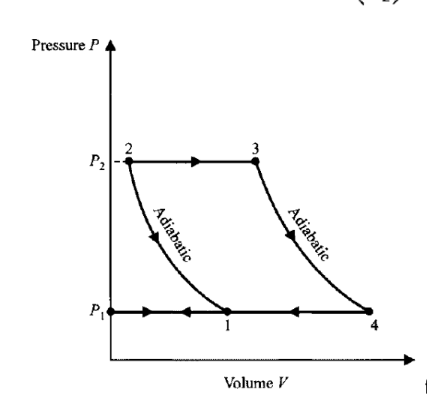
\includegraphics[width=0.5\textwidth]{diagrama.png}
    \label{fig:figura1}    
\end{figure}
    \begin{answer}[Punto 22]
        Partiendo de las ecuaciones canonicas de Hamilton:
        \begin{align*}
            \dot q_i &= \frac{\partial H}{\partial p_i} \quad \text{y} \quad \dot p_i = -\frac{\partial H}{\partial q_i} \quad  \frac{\partial H }{\partial t} = -\frac{\partial L}{\partial t} \quad (22.1)
        \end{align*}
        Y sea $u = u(q_i, p_i, t)$, entonces:
        \begin{align*}
            \frac{du}{dt} &= \frac{\partial u}{\partial q_i} \dot q_i + \frac{\partial u}{\partial p_i} \dot p_i + \frac{\partial u}{\partial t}\\
            &= \frac{\partial u}{\partial q_i} \frac{\partial H}{\partial p_i} - \frac{\partial u}{\partial p_i} \frac{\partial H}{\partial q_i} + \frac{\partial u}{\partial t}\\
            &= \left\{u, H\right\} + \frac{\partial u}{\partial t} \quad (22.2)
        \end{align*}

        Si definimos: $\pmb \eta \equiv (q_i(t), p_i(t))$, tal que $\dot {\pmb \eta} = (\dot q_i, \dot p_i)$, entonces:
        \begin{align*}
            \dot {\pmb \eta} &= \begin{pmatrix}
                \dot q_i \\
                \dot p_i \\
            \end{pmatrix} = \begin{pmatrix}
                \frac{\partial H}{\partial p_i} \\
                -\frac{\partial H}{\partial q_i} \\
            \end{pmatrix}\\
             &= \begin{pmatrix}
                0 & \mathbf 1\\
                -\mathbf 1 & 0\\
            \end{pmatrix} \begin{pmatrix}
                \frac{\partial H}{\partial q_i} \\
                \frac{\partial H}{\partial p_i} \\
            \end{pmatrix} 
            = J \frac{\partial H}{\partial \pmb \eta} = \tilde{\frac{\partial \pmb \eta}{\partial \pmb \eta}} J \frac{\partial H}{\partial \pmb \eta} \\
            &= \left\{\pmb \eta, H\right\} \quad  \Rightarrow 
        \end{align*}

        \begin{align*}
            \dot {\pmb \eta} = \left\{\pmb \eta, H\right\} \quad (22.2)
        \end{align*}
        Son las ecuaciones canonicas de Hamilton en corchetes de Poisson, con $\frac{\partial \pmb \eta}{\partial t} =0$, pues podemos notar que:
        \begin{align*}
            \left\{q_i, H \right\} = \tilde{\frac{\partial  q_i}{\partial \pmb \eta}} J \frac{\partial H}{\partial \pmb \eta} = \begin{pmatrix} 1 \\ 0 \end{pmatrix} \begin{pmatrix} 0 & 1 \\ -1 & 0 \end{pmatrix} \begin{pmatrix} \frac{\partial H}{\partial q_i} \\ \frac{\partial H}{\partial p_i} \end{pmatrix} = \frac{\partial H}{\partial p_i} = \dot q_i\\
        \end{align*}
        \begin{align*}
            \left\{p_i, H \right\} = \tilde{\frac{\partial  p_i}{\partial \pmb \eta}} J \frac{\partial H}{\partial \pmb \eta} = \begin{pmatrix} 0 \\ 1 \end{pmatrix} \begin{pmatrix} 0 & 1 \\ -1 & 0 \end{pmatrix} \begin{pmatrix} \frac{\partial H}{\partial q_i} \\ \frac{\partial H}{\partial p_i} \end{pmatrix} = -\frac{\partial H}{\partial q_i} = \dot p_i\\
        \end{align*}
        \begin{align*}
            \left\{H, H \right\} + \frac{\partial H}{\partial t}= \tilde{\frac{\partial  H}{\partial \pmb \eta}} J \frac{\partial H}{\partial \pmb \eta} = \begin{pmatrix} \frac{\partial H}{\partial q_i} \\ \frac{\partial H}{\partial p_i} \end{pmatrix} \begin{pmatrix} 0 & 1 \\ -1 & 0 \end{pmatrix} \begin{pmatrix} \frac{\partial H}{\partial q_i} \\ \frac{\partial H}{\partial p_i} \end{pmatrix} = \frac{d H}{d t}
        \end{align*}
    \end{answer}
    9. (a) Deduzca la expresión para la eficiencia de un motor de Carnot directamente de un diagrama TS (Temperatura vs Entropía). (b) Compare las eficiencias de los ciclos A y B de la Figura 2.
figura 2.

\begin{figure}[h]
    \centering
    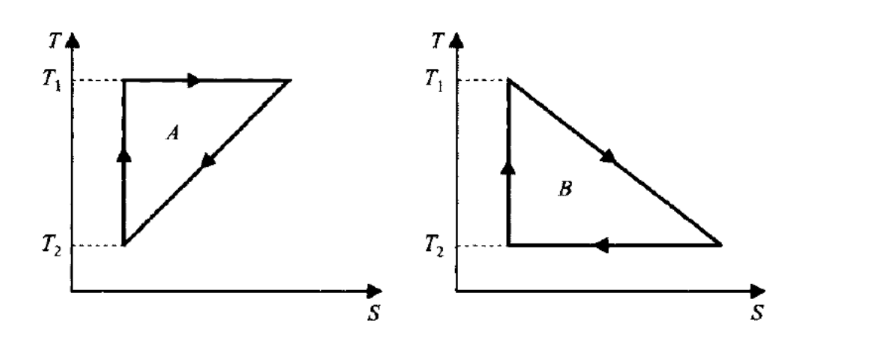
\includegraphics[width=0.5\textwidth]{diagram2.png}
    
    \label{fig:figura2}
\end{figure}
    \begin{answer}[Punto 23]
         
    \end{answer}


    10. La capacidad calorífica molar a campo magnético constante de un sólido paramagnético a bajas temperaturas varía con la temperatura y el campo según la relación
$$
C_{\mathscr{H}}=\frac{B+C \mathscr{H}}{T^2}+D T^2
$$
donde B, C y D son constantes. ¿Cuál es el cambio de entropía de n moles de material cuando la temperatura cambia de $\mathrm{T_i}$ a $T_f$ mientras que $\mathscr{H}_{0}$ permanece constante en el valor $\mathscr{H_0}$ 
    \begin{answer}[Punto 10]
        La entropia esta definida por:
        \begin{align*}
            dQ = TdS \quad &\Rightarrow \quad \left( \frac{dQ}{dT}\right)_{\mathscr{H}} = T \left(\frac{dS}{dT}\right)_\mathscr{H}\\
            &\Rightarrow \quad C_{\mathscr{H}} = T \left(\frac{dS}{dT}\right)_{\mathscr{H}}\\
            &\Rightarrow \quad dS = \frac{C_{\mathscr{H}}}{T}dT\\
            &\Rightarrow \quad dS = \left(\frac{B+C \mathscr{H}_0^2}{T^2}+D T^2\right)\frac{dT}{T}\\
            &\Rightarrow \quad S = \int_{T_i}^{T_f} \left(\frac{B+C \mathscr{H}_0^2}{T^2}+D T^2\right)\frac{dT}{T}\\
            &\Rightarrow \quad S = \int_{T_i}^{T_f} \left(\frac{B+C \mathscr{H}_0^2}{T^3}+D T\right)dT\\
            &\Rightarrow \quad S = \left[-\frac{B+C \mathscr{H}_0^2}{2T^2}+D \frac{T^2}{2}\right]_{T_i}^{T_f}\\
            &\Rightarrow \quad S = -\frac{B+C \mathscr{H}_0^2}{2T_f^2}+D \frac{T_f^2}{2} + \frac{B+C \mathscr{H}_0^2}{2T_i^2}-D \frac{T_i^2}{2}\\
            &\Rightarrow \quad S = \frac{B+C \mathscr{H}_0^2}{2}\left(\frac{1}{T_i^2}-\frac{1}{T_f^2}\right)+D \left(\frac{T_f^2}{2} -\frac{T_i^2}{2}\right)\\
            &\Rightarrow \quad S = \frac{B+C \mathscr{H}_0^2}{2}\left(\frac{T_f^2 - T_i^2}{T_i^2T_f^2}\right)+D \left(\frac{T_f^2 - T_i^2}{2}\right)\\
            &\Rightarrow \quad S =\frac{T_f^2 - T_i^2}2\left[ \left(\frac{B+C \mathscr{H}_0^2}{T_i^2T_f^2}\right)+D \left(T_f^2 - T_i^2\right)\right]\\
        \end{align*}
    \end{answer}
\end{document}